\chapter{Robust and Sparse Supervised Learning}\label{ch:SL}
%
%
In this chapter we now focus on supervised learning as described in \cref{sec:PSL}. 
\cite{bungert2021clip, bungert2021neural, kabri2023resolution, bungert2022bregman}
%
\section{Setting}
%
We are given a finite training set $\tset\subset\domain\times\OutSpace$. For a family of functions $f_\theta:\domain\to\OutSpace$ parameterized by $\theta\in \Theta$ we consider the empirical  minimization
%
\begin{align*}
\min_{\theta\in\Theta} \empLoss(\theta) 
\end{align*} 
%
where for a function $\ell:\OutSpace\times\OutSpace\to\R$ we define
\begin{align*}
\empLoss(\theta)  := \sum_{(x,y)\in \tset} \ell(f_\theta(x), y).
\end{align*}
%
Assuming that $\tset$ is sampled from a joint distribution $\pi$ on $\domain\times\OutSpace$ this approximates the infeasible population risk minimization
%
\begin{align*}
\int_{\domain\times\OutSpace} \ell(f_\theta(x), y) d\pi(x,y).
\end{align*}
%
In this thesis we focus on feed-forward neural networks, i.e., we consider layers of the form
%
\begin{align*}
\Phi(w, W, b)(z):= wz + \sigma(Wz + b)
\end{align*}
%
where $w\in\R$ models a residual connection, $W\in\R^{n\times n}$ is a weight matrix, $b\in\R^n$ a bias vector and $z\in\R^{m}$. We consider a concatenation of $L\in\N$ such layers, which then forms a neural network
%
\begin{align*}
f_\theta = \Phi^L\circ\ldots\circ\Phi^1
\end{align*} 
%
with parameters $\theta =(w_1,\ldots, w_L, W_1,\ldots, W_L, b_1,\ldots, b_L)\in\Theta$ and layers $\Phi^i := \Phi(w_i, W_i, b_i)$.
%
\paragraph{MLP}

\paragraph{Convolutions}

\paragraph{ResNets}

%
\section{Adversarial Stability}

%
\section{Sparsity via Bregman Iterations: \cite{bungert2022bregman}}

Intro sparsity blah blah
%
\begin{enumerate}
\item efficency
\item robustness
\item generalization
\end{enumerate}
%
\subsection{Preliminaries on Convex Analysis}

We first review some necessary concepts from convex analysis that allow us to introduce the framework in \cite{bungert2022bregman}. We refer to \cite{benning2018modern, rockafellar1997convex, bauschke2011convex} for a more exhaustive introduction to the topics.
%
The functional $\func$ is called lower semicontinuous if $\func(u)\leq\liminf_{n\to\infty}\func(u_n)$ holds for all sequences $(u_n)_{n\in\N}\subset\Param$ converging to $u$.
%
\begin{definition}{}{}
Given a Hilbert space $\Param$ and a functional $\func:\Param\to(-\infty,\infty]$.
%
\begin{enumerate}
\item The functional $\func$ is called convex, if
%
\begin{align}
    \func(\lambda\overline{\param}+(1-\lambda)\param)\leq
    \lambda\func(\overline{\param})
    +(1-\lambda)\func(\param),\quad\forall\lambda\in[0,1],\,\overline{\param},\param\in\Param.
\end{align}
%
\item The effective domain of $\func$ is defined as $\dom(\func):=\{\param\in\Param\st\func(\param)\neq\infty\}$ and $\func$ is called proper if $\dom(\func)\neq\emptyset$.
\end{enumerate} 
\end{definition}
%
%
In the following we want to consider functionals $J$ that are convex, but not necessarily differentiable. Therefor, we define the subdifferential.
%
\begin{definition}{}{}
of a convex {and proper} functional $\func:\Param\to(-\infty,\infty]$ at a point $\param\in\Param$ as
% ---------------------------------------------------------
\begin{align}
\label{eq:subgrad}
    \partial\func(\param) := \left\lbrace \sg\in\Param \st \func(\param) + \langle\sg,\overline{\param}-\param \rangle \leq \func(\overline{\param}),\;\forall\overline{\param}\in\Param\right\rbrace.
\end{align}
\end{definition}
% ---------------------------------------------------------
If $\func$ is differentiable, then the subdifferntial coincides with the classical gradient (or Fr\'echet derivative). We denote $\dom(\partial\func):=\{\param\in\Param\st\partial\func(\param)\neq\emptyset\}$ and observe that $\dom(\partial\func)\subset\dom(\func)$.

The main algorithm in this section are so-called Bregman iterations, for which we first define the Bregman distance.
%
\begin{definition}{Bregman Distance}{}
Let $\func:\Param\to(-\infty,\infty]$ be a proper, convex functional. Then we define for $\param\in\dom(\partial\func),\overline{\param}\in\Param$
% ---------------------------------------------------------
\begin{align}\label{eq:bregman_distance}
    D^\sg_\func(\overline{\param},\param) := \func(\overline \param)-\func({\param})-\langle\sg,\overline\param-{\param}\rangle,\quad\sg\in\partial\func(\param).
\end{align}
%
For $\sg\in\partial\func({\param})$ and $\overline\sg\in\partial\func(\overline{\param})$ we define the \emph{symmetric} Bregman distance as
\begin{align}
D^\mathrm{sym}_\func(\overline{\param},\param) := D^\sg_\func(\overline{\param},\param) + D^{\overline{\sg}}_\func(\param,\overline\param).
\end{align}
\end{definition}
% ---------------------------------------------------------
Intuitively, the Bregman distance $D^\sg_\func(\overline{\param},\param)$, measures the distance of $\func$ to its linearization around $\param$, see \cref{fig:Bregdist}.
%
\begin{figure}
\centering
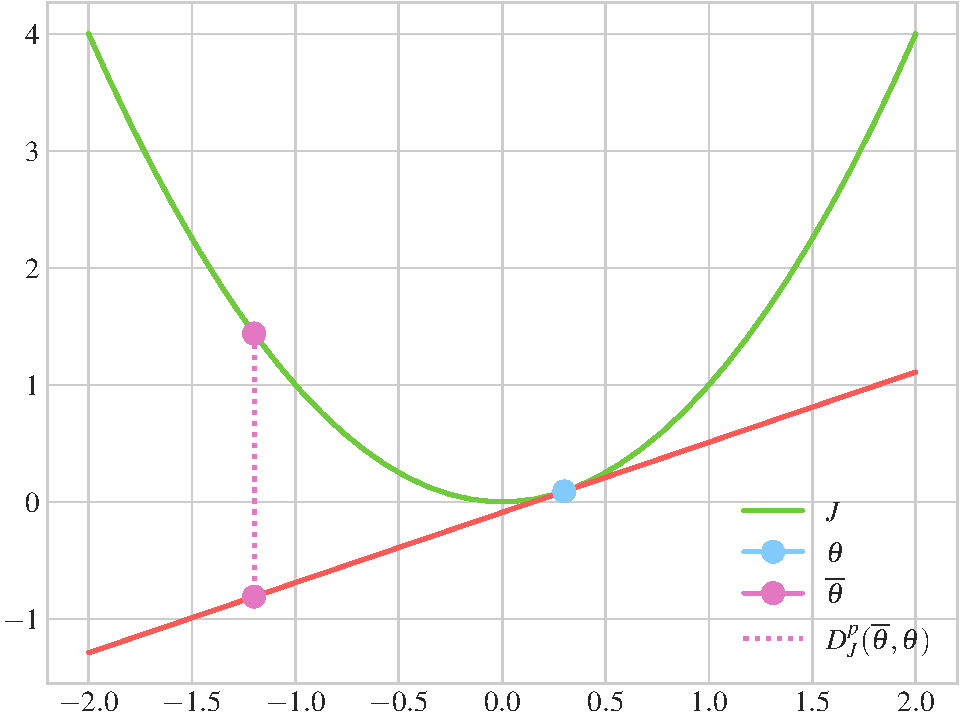
\includegraphics[width=.7\textwidth]{code/Bregman/lin_dist.pdf}
\caption{Visualization of the Bregman distance.}\label{fig:Bregdist}
\end{figure}
%
\begin{example}{}{ex:BregNorm}
For $\Param=\R^n$ and $J=\frac{1}{2}\norm{\cdot}_2^2$ we see that $\partial J(\param) = \{\param\}$ and therefore
%
\begin{align*}
D_J^p(\overline{\param}, \param) &= 
\frac{1}{2}\langle \overline\param,\overline\param\rangle - 
\frac{1}{2}\langle \param,\param\rangle - \langle \param, \overline\param-\param\rangle 
\\&=
\frac{1}{2}\langle \overline\param,\overline\param\rangle+
\frac{1}{2}\langle \param,\param\rangle -
\langle \param,\overline\param\rangle
\\&=
\frac{1}{2}\norm{\overline\param - \param}_2^2 = J(\overline\param - \param).
\end{align*}
\end{example}
%
We can easily see that in general it is neither definite, symmetric nor fulfills the triangle inequality, hence it is not a metric. 
However, it fulfills the two distance axioms
\begin{align}
D^\sg_\func(\overline{\param},\param) \geq 0,\quad D^\sg_\func(\param,\param)=0,\quad\forall\overline{\param}\in\Param,\param\in\dom(\partial\func).
\end{align}
%
The same holds for the symmetric Bregman distance, where additionally---as the name suggests---the symmetry property is fulfilled.
%
%
The last concept that is crucial in \cite{bungert2022bregman} is the so-called proximal operator.
%
\begin{definition}{}{}
Let $\func:\Param\to(-\infty,\infty]$  be convex, proper and lower semicontinuous functional, then we define the \emph{proximal operator} as
\begin{align}
    \prox{\func}(\overline{\param}) := \argmin_{\param\in\Param} \frac{1}{2}\norm{\param-\overline{\param}}^2 + \func(\param).
\end{align}
\end{definition}
%
%
\subsection{Bregman Iterations}
%
We first consider the following implicit Euler scheme, for a step size $\tau>0$
\begin{subequations}\label{eq:bregman_iteration}
\begin{align}
    \param^{(k+1)} &= \argmin_{\param\in\Param} D^{\sg^{(k)}}_\func(\param,\param^{(k)}) + \tau^{}\empLoss(\param), \\
    \sg^{(k+1)} &= \sg^{(k)} - \tau^{}\nabla\empLoss(\param^{(k+1)}) \in \partial \func(\param^{(k+1)})
\end{align}
\end{subequations}
%
which is known as the \emph{Bregman iteration} \cite{osher2005iterative}. The intuitive interpretation here is, that in each step we want to minimize $\empLoss$ while also being close to the previous iterate in terms of the Bregman distance induced by $J$. If $J=\frac{1}{2}\norm{\cdot}_2^2$ as in \cref{ex:BregNorm}


The time continuous flow for $\tau\to 0$ is known as the \emph{inverse scale space} flow \cite{burger2006nonlinear,burger2007inverse},
%
\begin{align*}
    \begin{cases}
        \dot{\sg}_t = - \nabla\empLoss(\param_t), \\
        \sg_t \in \partial \func(\param_t),
    \end{cases}
\end{align*}
%
\section{Resolution Stability}
%

